\chapter*{V1: Introduction}
\addcontentsline{toc}{chapter}{V1: Introduction}
\setcounter{chapter}{1}

\section*{V1a: Course Preview}
\addcontentsline{toc}{section}{V1a: Course Preview}
\setcounter{section}{1}

\subsection*{What is Cryptography?}
\begin{Definition}{Cryptography}{}
    \textbf{Cryptography} is about securing communications in the presence
    of \emph{malicious} adversaries.
\end{Definition}

\begin{figure}[!ht]
    \centering
    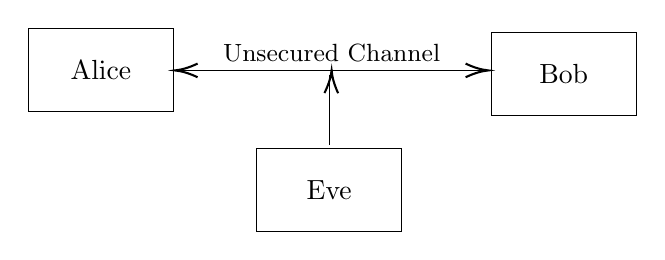
\begin{tikzpicture}[x=0.75pt,y=0.75pt,yscale=-1,xscale=1]
        %Shape: Rectangle [id:dp1673239703550864] 
        \draw   (10,10) -- (80,10) -- (80,50) -- (10,50) -- cycle ;
        %Straight Lines [id:da9805850481106809] 
        \draw    (82.67,30.33) -- (229.67,30.33) ;
        \draw [shift={(231.67,30.33)}, rotate = 180] [color={rgb, 255:red, 0; green, 0; blue, 0 }  ][line width=0.75]    (10.93,-3.29) .. controls (6.95,-1.4) and (3.31,-0.3) .. (0,0) .. controls (3.31,0.3) and (6.95,1.4) .. (10.93,3.29)   ;
        \draw [shift={(80.67,30.33)}, rotate = 0] [color={rgb, 255:red, 0; green, 0; blue, 0 }  ][line width=0.75]    (10.93,-3.29) .. controls (6.95,-1.4) and (3.31,-0.3) .. (0,0) .. controls (3.31,0.3) and (6.95,1.4) .. (10.93,3.29)   ;
        %Shape: Rectangle [id:dp26829412800555263] 
        \draw   (233,12) -- (303,12) -- (303,52) -- (233,52) -- cycle ;
        %Straight Lines [id:da5166974079328035] 
        \draw    (155,66.33) -- (155,32.33) ;
        \draw [shift={(156.17,30.33)}, rotate = 450.8] [color={rgb, 255:red, 0; green, 0; blue, 0 }  ][line width=0.75]    (10.93,-3.29) .. controls (6.95,-1.4) and (3.31,-0.3) .. (0,0) .. controls (3.31,0.3) and (6.95,1.4) .. (10.93,3.29)   ;
        %Shape: Rectangle [id:dp7316183888881436] 
        \draw   (120,68) -- (190,68) -- (190,108) -- (120,108) -- cycle ;
        % Text Node
        \draw (156.17,27.33) node [anchor=south] [inner sep=0.75pt]  [font=\small] [align=left] {Unsecured Channel};
        % Text Node
        \draw (45,30) node   [align=left] {Alice};
        % Text Node
        \draw (268,32) node   [align=left] {Bob};
        % Text Node
        \draw (155,88) node   [align=left] {Eve};
    \end{tikzpicture}
\end{figure}

In the basic communications model we have two parties: Alice and Bob. They
are exchanging messages over an \emph{unsecured} channel such as the internet.
By \emph{unsecured} we mean that their communications might be
under attack by an adversary who we call Eve, or eavesdropper.

Eve can certainly read data exchanged between Alice and Bob, but Eve
can also modify data, inject data,
delete data, and so on. Therefore, the term Eve can be a bit misleading since Eve
can do \emph{a lot} more than just eavesdrop. For
the remainder of the course,
when the term Eve is used please do not think of Eve
as an eavesdropper, but rather as a very powerful, malicious, unpredictable,
and evil adversary. What kind of security can Alice and Bob hope
to achieve in the presence of such strong adversaries?

\subsection*{Fundamental Goals of Cryptography}
\begin{enumerate}
    \item \emph{Confidentiality}: Keeping data secret from all but those
          authorized to see it.

              {\color{blue} When Alice
                  sends Bob a message, even though
                  Eve can read all the transmitted data, Alice
                  and Bob are the only parties
                  who can read the actual underlying message.
                  In practice, confidentiality
                  is achieved through the use of encryption.}
    \item \emph{Data integrity}: Ensuring data has not been altered by unauthorized
          means.

              {\color{blue} When Bob receives a message from Alice, Bob has
                  the assurance that the message wasn't modified during transmission.}
    \item \emph{Data origin authentication}: Corroborating the source of data.

              {\color{blue}
                  When Bob receives a message supposedly sent by Alice, Bob can verify that
                  the message indeed was sent by Alice.}
    \item \emph{Non-repudiation}: Preventing an entity from denying previous commitments or
          actions.

              {\color{blue} Broadly speaking, this
                  is preventing an entity from
                  denying previous commitments or actions. In
                  the physical world,
                  non-repudiation is provided through the use
                  of handwritten signatures. Cryptography though can be used to provide
                  the same security as handwritten signatures, but in the digital world.}
\end{enumerate}
We'll see in the remainder of the course that cryptography can be used to provide
confidentiality, data integrity, data origin authentication, and non-repudiation.

It should be evident that these four security services provided by
cryptography are very important in many applications where
sensitive data might be communicated or stored. Let's look
at some examples.

\begin{Example}{Email}{}
    Firstly, when Alice connects to the website, she needs the assurance that
    she really is visiting g-mail's website, not the website of an impersonator.
    Next, when she enters her email address and password, these are transmitted
    over the internet and so need to be secured through the use of encryption.
    Lastly, when Alice uploads and downloads emails, these are also transmitted
    over the internet and so have to be encrypted and authenticated.
\end{Example}
\begin{Example}{Online Shopping}{}
    Cryptography helps engender trust in e-commerce applications for both
    consumers and vendors.

    This is accomplished by encrypting and authenticating all sensitive financial
    and personal data that might be transmitted between Alice and Bob.
\end{Example}
\begin{Example}{Automatic Software Upgrades}{}
    Cryptography helps in guaranteeing the safety of automatic software upgrades.

    Imagine Microsoft broadcasting upgrades of its operating system to hundreds of millions
    of devices around the world.
    When such a device receives an upgrade, it needs the assurance that the
    software upgrade indeed is from Microsoft and hasn't been modified during
    transmission. In practice, these assurances are provided through the use
    of digital signatures.

    Note: Confidentiality is not required in this scenario because the software
    upgrades themselves are not considered to be private.
\end{Example}
\begin{Example}{Cell Phone Service}{}
    When you make a call on your cell phone the connection is established to a
    nearby cell phone tower. The cell phone tower needs the assurance that
    you have the authorization to use the cell phone service.
    Furthermore, your voice data needs to be encrypted and authenticated as it
    is transmitted over the air to the cell phone tower.
\end{Example}
\begin{Example}{WiFi}{}
    When you connect to a WiFi network, your cell phone has to authenticate itself to
    the WiFi router to prove that it has the authorization to use the WiFi
    service. Furthermore, all internet communications between
    your cell phone and the router have to be encrypted and authenticated.
\end{Example}
\begin{Example}{Bluetooth}{}
    When two devices such as your cell phone and
    your headset establish a Bluetooth connection this means that all data
    transmitted between the two devices is encrypted and authenticated using
    cryptographic mechanisms.
\end{Example}
\begin{Example}{Messaging}{}
    Cryptography is used to secure instant messaging, most famously by WhatsApp which
    provides very strong \emph{end-to-end encryption}. End-to-end encryption
    is when \emph{only} the two users who are exchanging messages can read them. In particular,
    WhatsApp itself cannot read the exchange messages.
\end{Example}
Hopefully, these examples convince the reader that cryptography
is extremely useful and important in securing all kinds of applications
where sensitive data might be communicated or stored.

One shouldn't think of Alice and Bob as human beings but rather as two communicating devices.

\begin{table}[!ht]
    \caption{Communicating Parties}
    \begin{tabularx}{0.9\linewidth}{@{}YYY@{}}
        \toprule
        \emph{Alice}       & \emph{Bob}      & \emph{Communications channel} \\
        \midrule
        person             & person          & telephone cable               \\
        person             & person          & cellular network              \\
        person             & website         & internet                      \\
        iPhone             & wireless router & wireless                      \\
        iPhone             & headphones      & wireless                      \\
        car's brakes       & another car     & wireless                      \\
        smart card         & bank machine    & financial network             \\
        smart meter        & energy provider & wireless                      \\
        military commander & satellite       & space
    \end{tabularx}
\end{table}

\subsection*{Secure Web Transactions}
\begin{Example}{Secure Web Transactions}{}
    Cryptography is used to secure web transactions via
    \emph{Transport Layer Security}.

    \begin{Definition}{Transport Layer Security (TLS)}{}
        The cryptographic protocol used by web browsers for secure web transactions
        for secure access to amazon, g-mail, Facebook, etc.
    \end{Definition}
    TLS is used to assure
    an individual user (\emph{client}) in this case Alice, of the
    authenticity of the website (\emph{server}),
    in this case g-mail, he
    or she is visiting, and to
    establish a \emph{secure communications channel}
    for the remainder of the session.

    All data communicated between Alice and the
    website need to be encrypted and authenticated
    which is accomplished using
    \emph{symmetric-key cryptography}.

    \begin{Definition}{Symmetric-key Cryptography}{}
        The \emph{client} and \emph{server}, a
        priori, share some \emph{secret} information
        $ k $, called a \emph{key}.
    \end{Definition}

    Once Alice and Bob have such a secret key, they can subsequently
    engage in secure communications by encrypting their messages with
    Advanced Encryption Standard (AES) and authenticating the
    resulting ciphertexts with HMAC.\@ We'll study AES and
    HMAC later on in the course.
\end{Example}
\underline{Question}: Alice and Bob establish the
shared secret key $ k $ in the first place?

Alice cannot simply select $ k $ and
transmit it over the internet to Bob because
then the eavesdropper would learn $ k $.

This is where \emph{public-key cryptography} is very useful.

\begin{Definition}{Public-key Cryptography}{}
    Communicating parties a priori, share
    some \emph{authenticated} (but non-secret) information.
\end{Definition}
Now, to establish a secret key, the client Alice selects the secret session key $ k $,
and encrypts it with the servers \emph{RSA public key}, and sends the
resulting ciphertext over the internet to Bob. Only Bob the server can decrypt the resulting
ciphertext, because decryption requires the use of the corresponding
RSA private key which only Bob knows. And so Bob decrypts the ciphertext
to recover $ k $, and $ k $ is known only to Alice and Bob.

\underline{Question}: How does Alice obtain an authentic copy
of the server's RSA public key?

Bob cannot just send the public key to Alice over the internet because Eve could
intercept this public key and replace it with her own public key.

This problem is solved using signature schemes.

\begin{Definition}{Signature Scheme}{}
    The server's RSA public key is \emph{signed} by a
    \emph{Certifying Authority} (CA) using the
    \textbf{RSA signature scheme}.
\end{Definition}
The client can verify the signature using the CA's RSA public verification key
which is embedded in Alice's browser.

In this way, the client obtains an authentic copy of the server's RSA public key.

\subsection*{The TLS protocol}
\begin{enumerate}
    \item When a client first visits
          a secured website, the server transmits its \emph{certificate} to the client.
          \begin{itemize}
              \item The certificate contains the server's identifying
                    information (e.g.\ website name and URL)
                    and \underline{RSA} a public key, and the \underline{RSA} signature
                    of a \emph{certifying authority}.
              \item The certifying authority (e.g.\ Verisign) is trusted
                    to carefully verify the server's identity before issuing the certificate.
          \end{itemize}
    \item Upon receipt of the certificate, the client \emph{verifies} the
          signature using the certifying authority’s public key,
          which is embedded in the browser. A successful
          verification confirms the \emph{authenticity} of the server and
          of its RSA public key
    \item The client selects a random \emph{session key} $ k $, \emph{encrypts} it
          with the server’s RSA public key, and transmits the
          resulting ciphertext to the server.
    \item The server \emph{decrypts} the ciphertext to obtain the
          session key, which is then used with symmetric-key schemes
          to \emph{encrypt} (e.g.\ with AES) and \emph{authenticate}
          (e.g.\ with HMAC) all sensitive data exchanged for the remainder of the session.
    \item The establishment of a secure link is indicated by a
          \emph{closed padlock} in the browser. Clicking on this icon
          reveals the server’s certificate and information about
          the certifying authority.
\end{enumerate}

TLS is one of the most successful security technologies ever deployed, but
is TLS \emph{really} secure?

\subsection*{TLS\@: Potential Vulnerabilities}

\begin{enumerate}
    \item The cryptography is weak (e.g.\ AES, HMAC, RSA).

              {\color{blue} Recall from MATH 135 that the security of
                  RSA is based on the presumed difficulty of factoring large numbers. No one
                  knows how to factor large numbers efficiently today, however there is a
                  possibility that such an algorithm might be discovered tomorrow.}
    \item \emph{Quantum attacks} on the underlying crpytography.

              {\color{blue} We do know how to factor large numbers very
                  quickly on quantum computers,although it isn't known as yet whether one
                  can actually build large-scale quantum computers.}
    \item Weak random number generation.

              {\color{blue} In TLS, browsers select random
                  session keys. In practice, selecting random numbers is a very difficult
                  problem in software applications.

                  Many deployments of TLS have been found to be insecure in the past 20 years
                  due to poor random number generation.}
    \item Issuance of fraudulent certificates.
          \begin{itemize}
              \item In 2001, Verisign erroneously issued two Class 3
                    code-signing certificates to a person masquerading as a Microsoft
                    representative.

                        {\color{blue}In principle, this person could have generated malware,
                            signed it with its RSA private key, broadcast this malware to computers around
                            the world, and the computers would have accepted the malware as originating
                            from Microsoft. This problem was caused by \emph{human error}, not due to any
                            deficiency in the underlying cryptography.}
          \end{itemize}
    \item Software bugs (both inadvertent and malicious).
    \item \emph{Phishing} attacks.
    \item TLS only protects data during transit. It does
          \emph{not} protect your data when it is collected at the server.
          \begin{itemize}
              \item Many servers store large amounts of credit card data and other
                    personal information.
          \end{itemize}
    \item The National Security Agency (NSA).

          \begin{figure}[!ht]
              \centering
              \includegraphics[width=0.75\textwidth]{nsa.jpg}
          \end{figure}

          {\color{blue} We give an example from the Snowden revelations. In
          2013, Edward Snowden, an NSA employee, leaked a large number of highly
          classified NSA documents to the press. One such document was headed
          ``Current Efforts Google.''

          On the left, the
          slide showed the public internet. So it showed users connecting using TLS, also
          known as SSL, to Google's front-end servers. So all data exchange between
          users and Google servers are protected using TLS.\@

          However, the slide also had the statement ``SSL added and
          removed here'' with a smiley face, and the note that ``traffic in cleartext
          here.''

          So Google's front-end servers would
          then transmit the decrypted data
          to its data centers around the world. These
          transmissions took place in
          the so-called Google cloud, where the data
          centers were connected by private
          links. In particular, the data transmitted
          between these links were not
          encrypted. As it turns out, NSA had access
          to one of these links between
          two Google data centers and NSA was capturing
          and storing gigantic amounts
          of user data transmitted between these two
          data centers.

          Therefore, even though TLS
          itself was secure, what was not secure was
          the way in which data was stored
          and transmitted in Google's back end.}
\end{enumerate}

\subsection*{Cryptography in Context}

These examples of potential vulnerabilities
in TLS tell us that cryptography must be studied in a context, and that broader
context is information security, now known as Cybersecurity. Cybersecurity
is a very broad field and it's difficult to give it a precise definition.
Nonetheless, here's one attempt.

\begin{Definition}{Cybersecrity}{}
    \textbf{Cybersecurity} is comprised of the concepts,
    technical measures, and administrative measures used to protect networks,
    computers, programs and data from deliberate or inadvertent unauthorized
    access, disclosure, manipulation, loss or use.

    Also known as \emph{information security}.
\end{Definition}

\begin{table}[!ht]
    \caption{Cybersecrity Includes the Study of:}
    \begin{tabularx}{0.9\linewidth}{@{}YYY@{}}
        \emph{Computer security}    & \emph{Network security}               & \emph{Software security}                   \\
        \midrule
        Security models and polices & Internet Protocols and their security & Detecting and preventing buffer overflows  \\
        Secure operating systems    & Viruses and worms                     & Programming languages and compilers        \\
        Virus protection            & Denial-of-service (DoS) attacks       & Specifying and enforcing security policies \\
        Auditing mechanisms         & Firewalls                             & Digital rights management                  \\
        Risk analysis               & Intrusion detection systems           & Code obfuscation                           \\
        Risk management             & Wireless communications               & Software tamper resistance                 \\
                                    &                                       & Trusted computing
    \end{tabularx}
\end{table}

\subsection*{Cryptography $ \neq $ Cybersecrity}
\begin{itemize}
    \item Cryptography provides some mathematical tools that can
          assist with the provision of cybersecurity services. It is a \emph{small},
          albeit an \emph{indispensable}, part of a complete security solution.
    \item \emph{Security is a chain}
          \begin{itemize}
              \item Weak links become targets; one flaw is all it takes.
              \item Cryptography is usually not the weakest link. However,
                    when the cryptography fails the damage can be catastrophic.
              \item This course will focus on cryptography.
          \end{itemize}
\end{itemize}

\subsection*{Syllabus}
\begin{minipage}{0.45\textwidth}
    \textbf{Cryptography primitives}
    \begin{itemize}
        \item Symmetric-key encryption
        \item Hash functions
        \item Message authentication
        \item Authenticated encryption
        \item Public-key encryption
        \item Signature schemes
        \item RSA
        \item Elliptic curve cryptography
        \item Key establishment
        \item Post-quantum cryptography
    \end{itemize}
\end{minipage}
\begin{minipage}{0.45\textwidth}
    \textbf{Cryptography deployments}
    \begin{itemize}
        \item IEEE 802.11 WEP/WPA2
        \item Google's KMS
        \item GSM security
        \item QQ browser
        \item FIDO U2F
        \item Bluetooth security
        \item Key management (PKIs)
        \item Web security protocols (TLS)
        \item Signal protocol (WhatsApp)
        \item Cryptocurrencies (Bitcoin)
    \end{itemize}
\end{minipage}
